\chapter{绪论}
\label{chap:1}
\section{研究背景与研究意义}

超高真空（Ultra-High Vacuum, UHV，通常指压力低于 $10^{-6}\,\mathrm{Pa}$ 的真空环境）是现代高端科学实验与先进制造技术的重要基础条件\cite{arpornthipVacuumpressureMeasurementUsing2012,成永军基于7Li冷原子操控的超高真空测量2024,贾文杰基于冷原子的量子真空计量技术研究进展2021,张苏钊基于磁光阱中6Li冷原子的真空度测量2022}。在基础科学领域，例如冷原子物理、量子信息技术、精密光谱测量以及基本常数测定等实验中，超高真空环境是获得长相干时间和高信噪比测量结果的前提条件\cite{barkerAccurateMeasurementLoss2023}。在粒子物理与加速器工程中，束流管道必须维持极低的气体密度，以减少粒子与残余气体分子的碰撞，从而避免能量损失及束流不稳定现象\cite{barkerPreciseQuantumMeasurement2022}。在航天推进系统、精密仪器制造以及表面科学分析（如扫描隧道显微镜、电子束曝光）等领域，稳定、可靠的超高真空测量同样发挥着关键作用\cite{barkerPreciseQuantumMeasurement2022}。因此，研发高精度、可溯源且对被测系统扰动较小的超高真空测量技术具有重要的现实意义和工程价值。

目前，超高真空测量领域广泛采用真空电离规作为主要测量手段，典型代表包括热阴极电离规和冷阴极电离规。然而，传统电离规在高精度测量与长期稳定运行方面仍存在若干固有局限，例如气体解吸效应、软 X 射线效应以及高温灯丝热辐射等问题\cite{bayardExtensionLowPressure1950}。这些因素会引入附加误差或背景信号，进而影响测量结果的准确性与系统运行的稳定性。

近年来发展起来的基于冷原子碰撞损失机制的真空测量技术，其核心思想在于利用冷原子与背景气体分子之间的弹性或非弹性碰撞这一内禀微观过程，实现对环境压强的量子化测量。在超高真空条件下，被俘获冷原子因与背景气体分子发生碰撞而逃逸出势阱，从而表现为原子数的指数衰减，其衰减速率 $\Gamma$ 与背景气体数密度 $n$ 之间满足线性关系
\[
n = \frac{\Gamma}{L},
\]
其中 $L$ 为损失率系数（loss-rate coefficient）。
结合理想气体状态方程
\[
P = nkT,
\]
可得到压强与原子损失率之间的直接关系\cite{barkerPreciseQuantumMeasurement2022}
\[
P = \frac{\Gamma}{L} k T.
\]

其中，损失率系数 $L$ 由原子—分子散射截面及相对速度分布决定，本质上仅依赖于微观相互作用势等基本物理参数，可通过第一性原理计算获得；玻尔兹曼常数 $k$ 为已知物理常数。因此，通过精确测量原子数衰减速率 $\Gamma$ 及环境温度 $T$，即可实现对环境压强 $P$ 的反演求解。

原子数衰减率的测量目前主要包含两种方法，其基本测量流程如下。首先，经过预冷却的原子蒸汽被囚禁于三维磁光阱中，衰减率测量过程可在磁光阱或磁阱内分别实施。第一种方法是在三维磁光阱中直接监测原子数的衰减过程，利用原子荧光强度表征原子数密度，通过获取荧光强度随时间的演化曲线，拟合得到原子数衰减速率$\Gamma$，如图\ref{fig:ch1-5}。该方法测量效率较高，能够快速获得衰减曲线，但原子与背景气体的碰撞截面计算较为复杂，现阶段仍缺乏精确的理论计算方法。

\begin{figure}[htbp] \centering 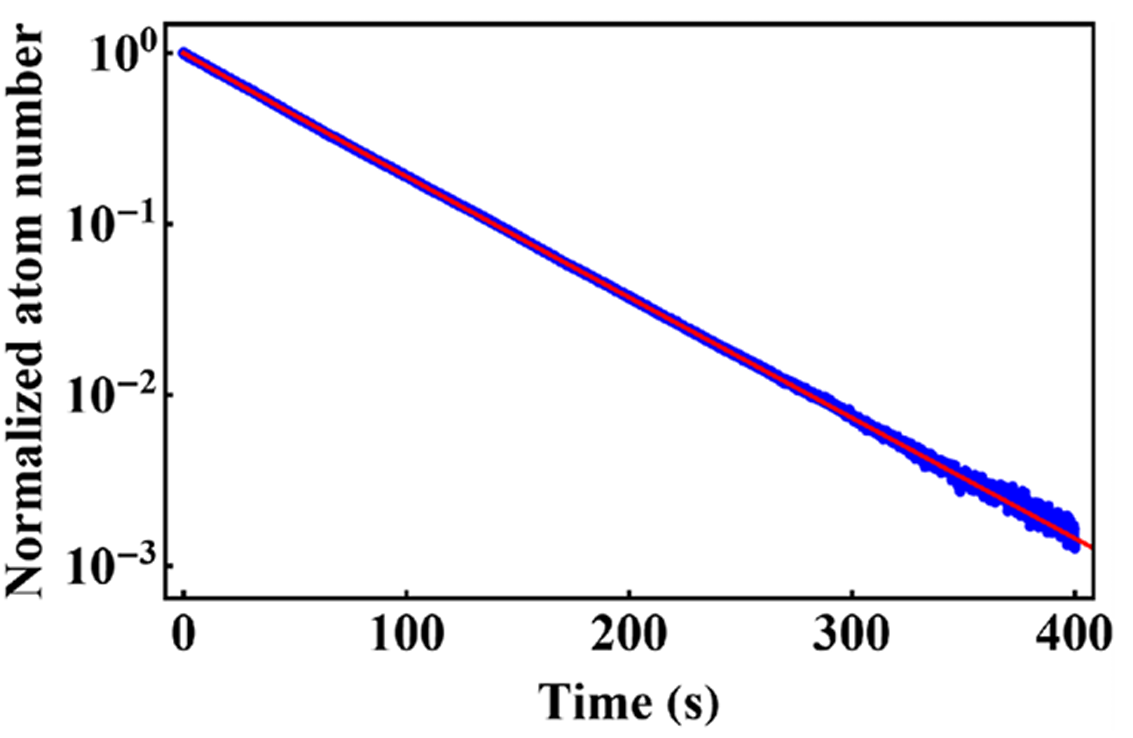
\includegraphics[width=0.5\linewidth]{figs/ch1-5.png} \caption{磁光阱中原子数衰减曲线\cite{zhangVacuumPressureMeasurement2023}} 
	\label{fig:ch1-5} 
\end{figure}

第二种方法则是将冷却后的原子从三维磁光阱装载至磁阱中，由于磁阱内不存在照射光束，原子无法产生荧光信号；待原子在磁阱中经历指定时间的数目衰减后，再将其重新装载回三维磁光阱进行荧光检测，通过对比不同时刻的荧光强度变化拟合出衰减速率$\Gamma$，如图\ref{fig:ch1-6}。此种方法的优势在于磁阱中原子与背景气体的碰撞截面物理图像明确、计算精度更高，不足之处是测量周期较长，需要对多个时间节点的原子数进行重复测量。

\begin{figure}[htbp] \centering 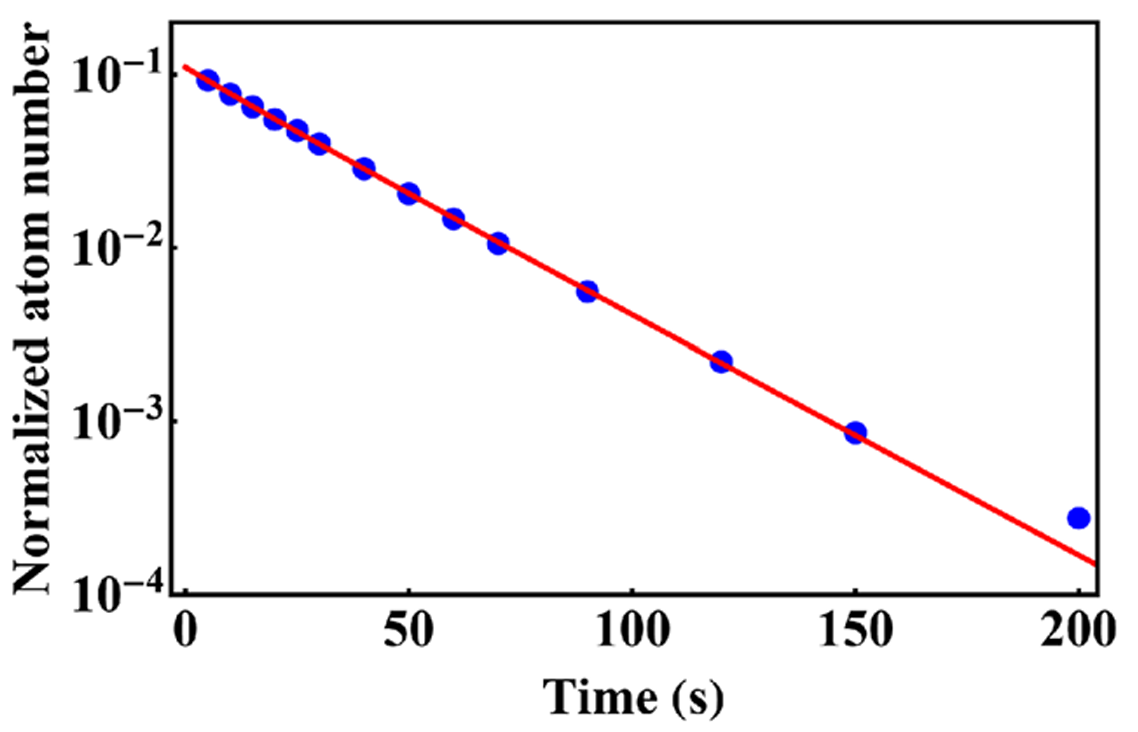
\includegraphics[width=0.5\linewidth]{figs/ch1-6.png} \caption{磁阱中原子数衰减曲线\cite{zhangVacuumPressureMeasurement2023}} 
	\label{fig:ch1-6} 
\end{figure}

由于该方法直接建立在微观散射动力学之上，避免了传统电离规中与电子发射、气体种类依赖等相关的系统误差来源，在原理上具有更高的准确度与长期稳定性。同时，其测量结果可溯源至基本物理常数与第一性原理计算，因而具备发展为新一代初级真空计量标准的潜力。


冷原子真空测量技术的发展可追溯至20世纪80年代激光冷却与俘获技术的突破。1987年磁光阱（Magneto-Optical Trap, MOT）的发明首次实现了对中性原子的稳定空间俘获，使原子样品能够在超高真空环境中长时间存留。随后研究逐步表明，原子俘获寿命与背景气体压强之间存在直接关联关系\cite{bjorkholmCollisionlimitedLifetimesAtom1988}，这一认识为基于碰撞损失机制的真空测量方法奠定了关键实验基础。

进入2010年代，随着激光系统稳定性的提升以及原子-分子碰撞截面计算精度的显著提高，相关研究由早期的定性关联分析逐步发展为定量模型构建，开始系统探索利用冷原子俘获寿命实现真空计量的可行性\cite{arpornthipVacuumpressureMeasurementUsing2012}。这一阶段标志着该技术从基础原子物理研究向计量应用方向的初步过渡。

美国国家标准与技术研究院（National Institute of Standards and Technology, NIST）在该领域开展了系统性研究，提出并实现了基于冷原子碰撞动力学的超高及极高真空量子标准体系。其核心思想是通过测量俘获原子的损失速率，并结合第一性原理计算得到的碰撞损失率系数，实现压力对基本物理常数的可溯源测量\cite{scherschligtDevelopmentNewUHV2017,barkerAccurateMeasurementLoss2023,barkerPreciseQuantumMeasurement2022,eckelEffectGlancingCollisions2025}。基于该原理，NIST构建了以铷原子为传感介质的实验室级量子真空计量装置，如图\ref{fig:ch1-1}所示。相关研究围绕碰撞截面的精确计算、原子损失模型修正、系统误差来源分析以及测量不确定度评定等关键问题展开，逐步建立了完整的量子真空计量框架。

\begin{figure}[htbp] \centering 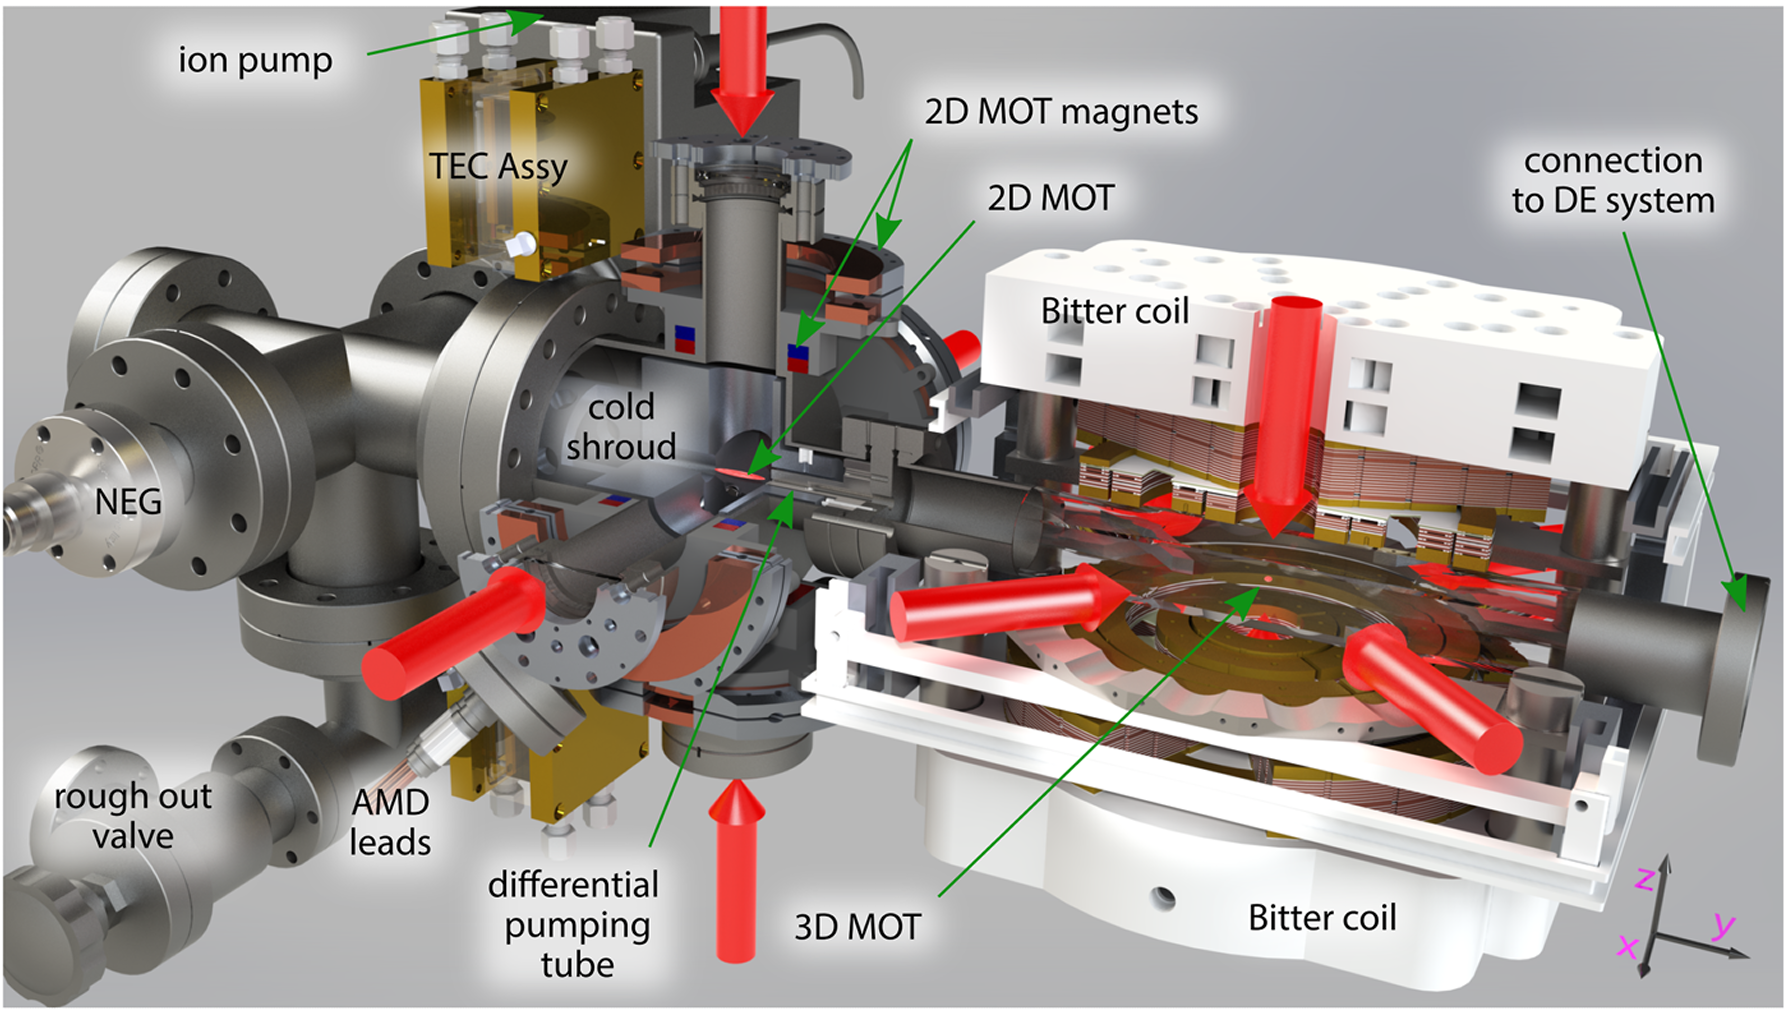
\includegraphics[width=0.5\linewidth]{figs/ch1-1.png} \caption{NIST实验室级量子真空计量装置\cite{barkerPreciseQuantumMeasurement2022}} 
\label{fig:ch1-1} 
\end{figure}

在工程实现方面，NIST进一步发展了基于锂原子的便携式冷原子真空标准装置\cite{barkerPreciseQuantumMeasurement2022,ehingerComparisonTwoMultiplexed2022}，如图\ref{fig:ch1-2}所示。通过引入紧凑型激光系统、永磁体磁场结构以及集成化光学模块设计，显著降低了系统体积与功耗，为现场应用与工程化部署提供了重要技术验证。

\begin{figure}[htbp] \centering 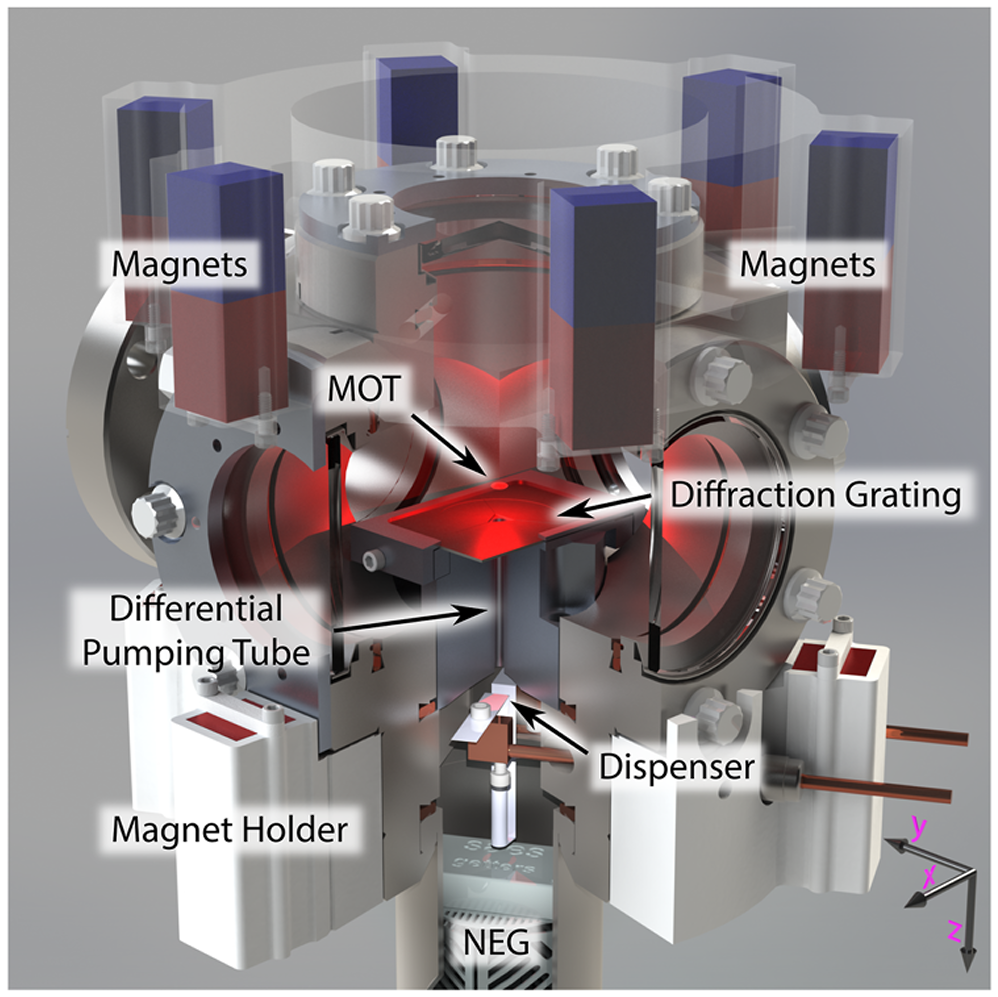
\includegraphics[width=0.5\linewidth]{figs/ch1-2.png} \caption{NIST基于锂原子的便携式冷原子真空标准装置\cite{barkerPreciseQuantumMeasurement2022}} \label{fig:ch1-2} \end{figure}

除NIST外，加拿大英属哥伦比亚大学（University of British Columbia, UBC）亦开展了系统研究，构建了基于铷原子的量子真空计量实验平台，如图\ref{fig:ch1-3}所示。其研究重点在于冷原子损失机制的精确建模以及多组分气体环境下的响应特性分析，同时对小型化冷原子真空计量装置进行了探索\cite{boothUniversalityQuantumDiffractive2019,shenDevelopmentColdAtom2022,shenRealizationUniversalQuantum2020,waldockProgressPortableColdatom2022}。此外，欧洲部分计量机构和研究团队亦对基于冷原子的量子真空计量方法开展了相关研究\cite{makhalovVacuumGaugeBased2017,halbeyDesignAdvancesDual2025}，为该技术纳入国际计量标准体系提供了重要的理论与实验支撑。

\begin{figure}[htbp] \centering 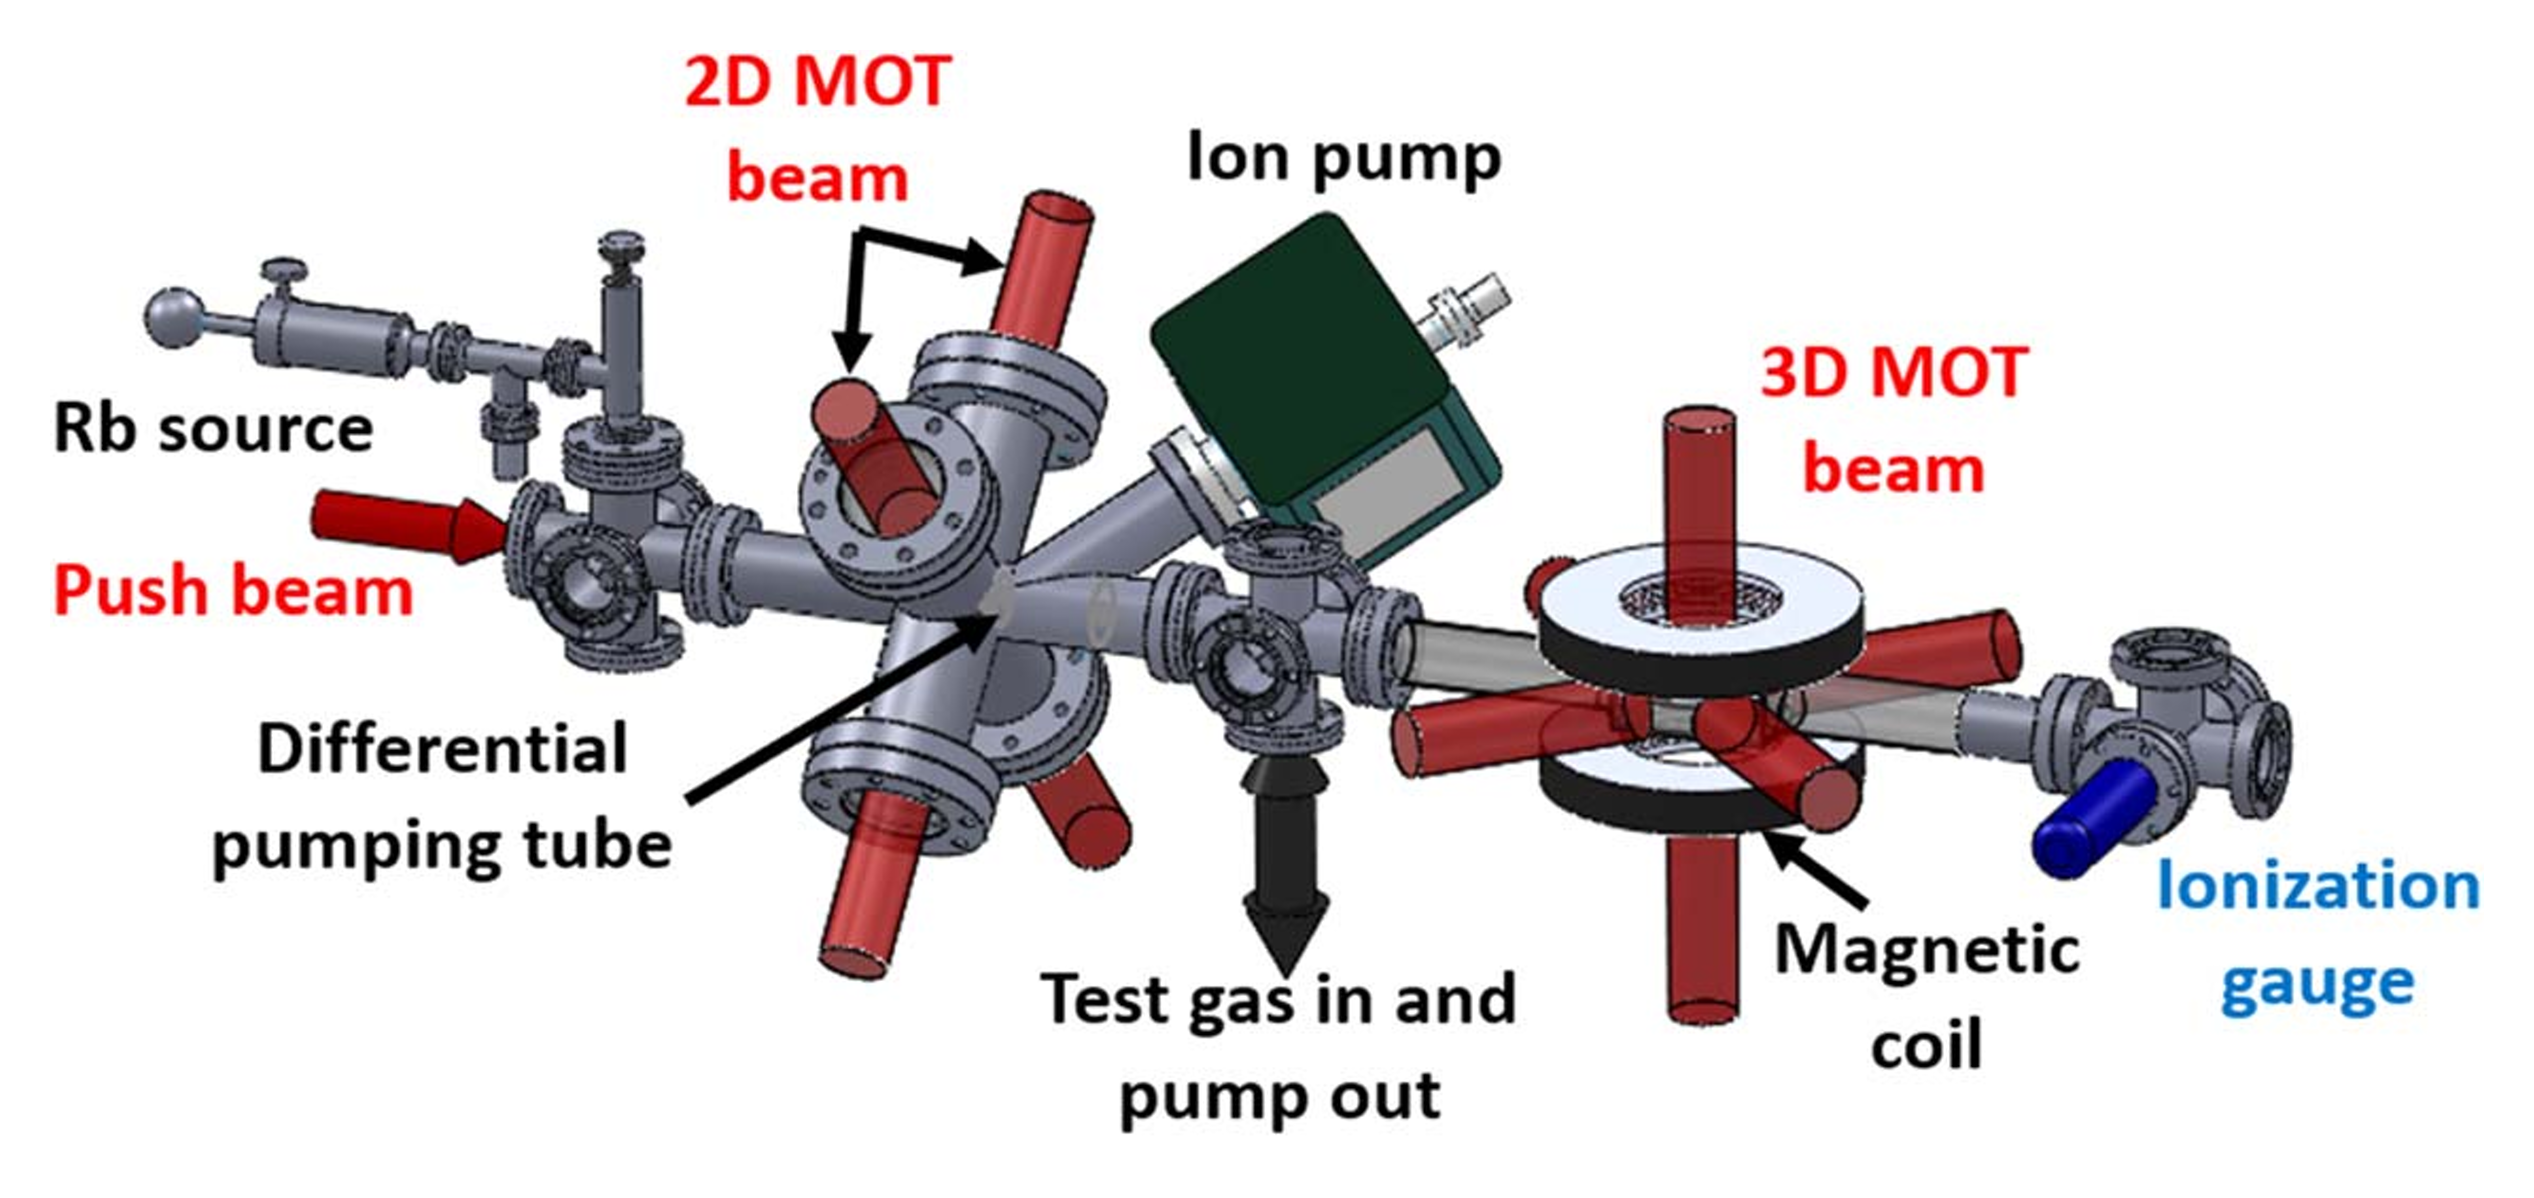
\includegraphics[width=0.6\linewidth]{figs/ch1-3.png} \caption{UBC基于铷原子的量子真空计量方案\cite{boothUniversalityQuantumDiffractive2019}} \label{fig:ch1-3} 
\end{figure}

在国内，冷原子真空计量研究同样发展迅速。以兰州空间技术物理研究所和华东师范大学等单位为代表的研究团队，围绕基于锂冷原子的真空计量方法开展了系统性研究\cite{fengImprovedDesignMagnetic2025,zhangVacuumPressureMeasurement2023,张苏钊基于磁光阱中6Li冷原子的真空度测量2022,成永军基于7Li冷原子操控的超高真空测量2024}，如图\ref{fig:ch1-4}。主要内容包括原子损失率与背景气体压强之间的定量标定、不同气体组分下灵敏度系数的分析以及系统不确定度评估等。在实验实现层面，国内已建立较为成熟的冷原子实验平台并取得阶段性进展，但在装置便携化设计、系统工程化集成以及长期稳定运行能力等方面仍有进一步提升空间。

\begin{figure}[htbp] \centering 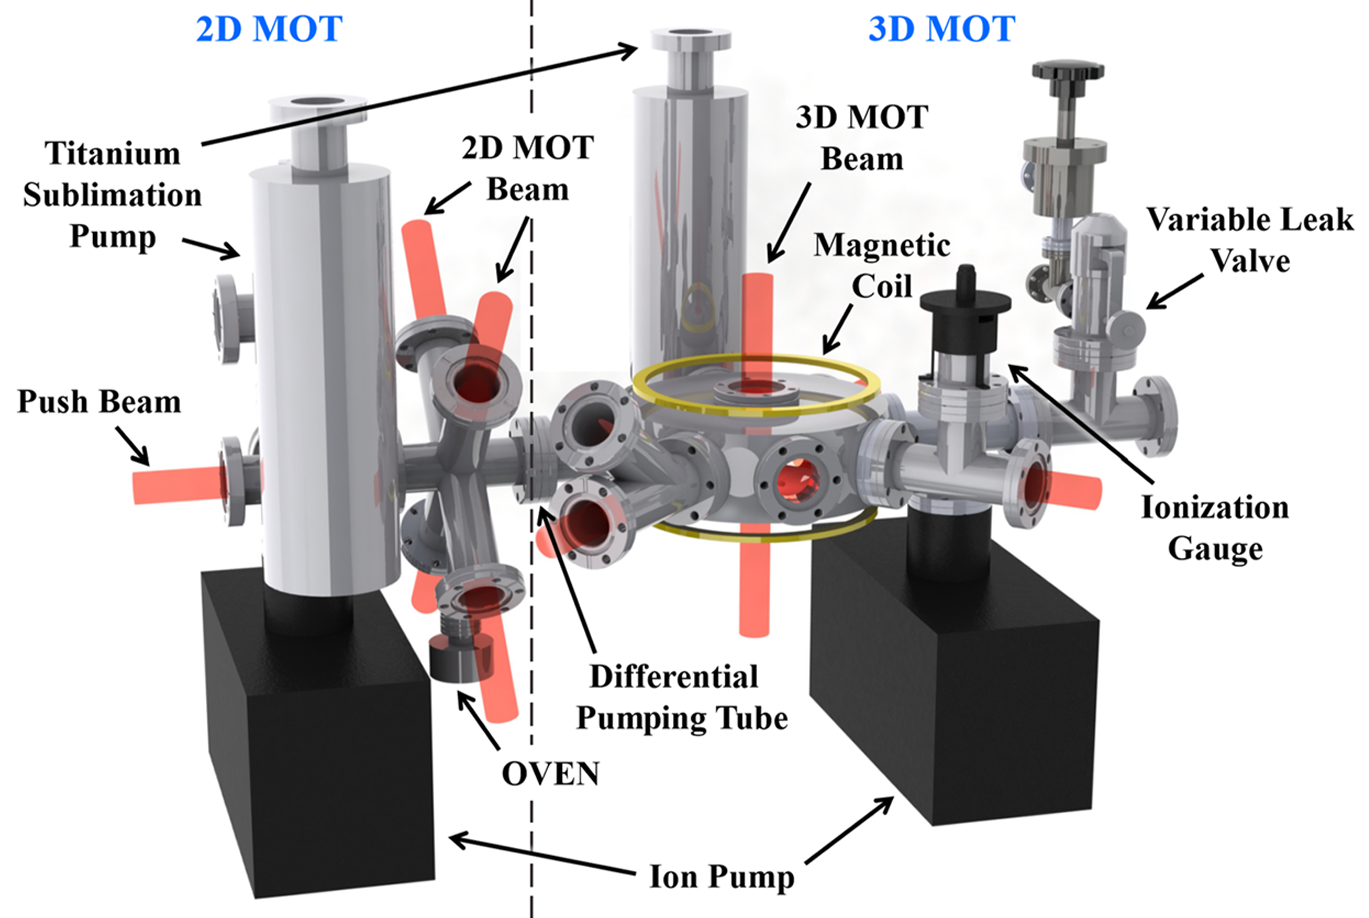
\includegraphics[width=0.6\linewidth]{figs/ch1-4.png} \caption{兰州空间技术物理研究所基于锂原子的实验室级量子真空计量方案\cite{zhangVacuumPressureMeasurement2023}} \label{fig:ch1-4} 
\end{figure}


综上所述，冷原子真空测量技术在物理机理验证与计量模型构建方面已趋于成熟，但在工程化实现与实际应用推广方面仍面临挑战，尤其体现在系统小型化、结构集成度以及长期稳定性等关键指标尚未完全定型。因此，依托中科院精密测量院在冷原子量子技术领域的研究基础，开展面向工程应用的小型化冷原子真空测量装置设计与测试研究，对于提升我国在量子真空计量领域的自主创新能力具有重要意义。

\section{研究内容和论文结构安排}

本课题围绕“小型化冷原子真空计量系统磁光阱装载实验”这一核心目标展开研究。冷原子真空计量技术利用原子与背景气体碰撞导致的损失过程来反演真空压强，其测量结果具有良好的可溯源性与物理可靠性。然而，传统冷原子实验装置通常体积较大、结构复杂，限制了该技术在实际应用场景中的推广。因此，本研究在既有理论模型与实验原理的基础上，重点探索冷原子真空测量系统的小型化实现方案，并通过系统实验对其性能进行验证。

本研究的核心思路是，在保证冷原子俘获与寿命测量条件的前提下，通过系统结构优化与实验流程改进，实现装置的紧凑化设计与稳定运行。与侧重计量标准建立或基本原理验证的研究工作相比，本课题更加关注系统工程实现过程，强调装置结构的可实现性与应用适配能力，从而为冷原子真空测量技术向实际工程应用过渡提供实验依据和技术参考。

在系统设计方面，本研究从光学系统、磁场系统以及真空系统三个方面对实验装置进行了整体优化。

在光学系统设计方面，引入小型化光路技术，对整体光路结构进行紧凑布局设计。通过合理采用分光与合束结构优化光束传输路径，在降低系统空间占用的同时保证光束的准直质量与功率稳定性，从而满足磁光阱对激光参数的要求。

在磁场系统设计方面，本研究采用永磁体与电磁线圈相结合的复合磁场结构，以产生磁光阱与磁阱所需的四极磁场梯度。与传统纯电磁线圈方案相比，该结构能够有效避免水冷系统带来的能耗问题与结构复杂性，从而显著降低系统体积与功率需求。同时，通过磁路设计与磁场分布仿真，对磁场梯度和空间分布进行优化，使其满足原子俘获条件，并兼顾系统调节能力与装配精度要求。

在真空系统设计方面，实验装置在保证小型化结构的同时兼顾光学访问需求。通过合理布置腔体视窗位置与抽气接口，在结构紧凑性与抽气效率之间取得平衡，从而保证系统能够满足冷原子实验所需的超高真空环境。

在系统测试方面，首先开展冷原子磁光阱俘获实验，包括原子云形态观察、荧光信号测量以及俘获原子数估算，以验证实验系统能够稳定实现原子俘获。之后会进行原子寿命测量实验，通过记录磁阱中原子数随时间的衰减曲线提取原子损失率参数，并建立其与背景气体压强之间的关系。最后将测量结果与传统电离规读数进行对比分析，以评估系统测量结果的一致性与重复性。通过多组实验数据的统计分析，对系统可能存在的误差来源进行讨论，并提出相应的改进方案。

通过上述研究工作，本课题完成了从系统设计、实验实现到性能验证的完整研究过程，突出了工程实践特点，为小型化冷原子真空测量系统的进一步发展提供了实验依据与技术参考。

本文的结构安排如下：第一章回顾冷原子真空计量技术的发展历程，总结国内外相关研究进展，并明确本研究的目标与定位。第二章介绍实验装置各组成部分的基本原理与设计方案，包括真空系统、激光系统和磁场系统的具体构建。第三章阐述磁光阱装载实验及实验结果。


